% CSWO-Bench final report (University of Oulu NLP course 2026, project 16).
% Compile: pdflatex report && bibtex report && pdflatex report && pdflatex report   (Overleaf: pdfLaTeX)
\documentclass{article}

\usepackage[utf8]{inputenc}
\usepackage[T1]{fontenc}
\usepackage{lmodern}
\usepackage{amsmath, amssymb}
\usepackage{booktabs}
\usepackage{graphicx}
\usepackage{xcolor}
\PassOptionsToPackage{hyphens}{url}   % long model ids may break at hyphens
\usepackage[colorlinks=true, linkcolor=black, citecolor=black, urlcolor=blue!50!black]{hyperref}
\usepackage{enumitem}
\setlist{nosep}
\graphicspath{{figures/}}

% red = still to fill in before submission
\newcommand{\fillin}[1]{\textcolor{red}{[#1]}}

\title{CSWO-Bench: A Multilingual Multimodal Benchmark of Citizen Science Water Observations}
\author{Eloi Mas Marti (2605397) \and Sam Brumwell (2605285) \and Finn Ullrich (2605284)}
\date{University of Oulu, Natural Language Processing 2026 \\ Course Project 16, proposed by Moinul Islam \\[4pt]
Code and data: \url{https://github.com/notEloiMm/cswo-bench} \\[4pt] \today}

\begin{document}
\maketitle

\section{Abstract}
CSWO-Bench is a benchmark regarding citizen-science water observations. Here, data is sampled across six different platforms,
harmonized and put into one singular schema. In total, this dataset contains 225,145 records.
This report consists of the results of specifications 2--9 (corpus, statistics, extraction,
gold set, agreement, baselines and image--text consistency), the bias audit of specification 11, and the literature
and limitations of specification 14.

\section{Introduction}

Volunteers can report states of different water-bodies, and upload them to one of many citizen-science platforms.
Each platform has its own schema, licence and language. We chose six of them: iNaturalist, CrowdWater~\cite{seibert2019crowdwater}, EyeOnWater, and 
three platforms published through GBIF~\cite{gbif}. We only kept open licences (CC0, CC-BY, ODbL, EyeOnWater's open policy) - each record
carries its licence and provenance. The next sections cover the project specifications.
\section{Spec 2 --- Harmonised corpus}

All sources were mapped into one schema containing note, English translation, photo URLs, date, coordinates rounded to 1\,km,
country, water-body type, labels, licence, provenance, hashed user id. The language was identified with
lingua and notes were translated to English with OPUS-MT~\cite{tiedemann2020opusmt} and
NLLB-200~\cite{nllb2022}, with an automatic check for empty, looping, truncated and hallucinated output.
We masked personal names, e-mails and typed coordinates in notes.

\begin{table}[htbp]
\centering\small
\caption{Records per platform and modality (\%).}
\label{tab:platforms}
\resizebox{\columnwidth}{!}{%
\begin{tabular}{lrrrrl}
\toprule
Platform & Records & Text only & Image only & Both & Main languages \\
\midrule
iNaturalist & 85{,}899 & 4.3 & 76.9 & 18.7 & en \\
CrowdWater & 65{,}892 & 0.4 & 78.0 & 21.5 & en, de, et, es \\
Artportalen & 28{,}223 & 100 & 0 & 0 & sv \\
EyeOnWater & 26{,}758 & 0 & 100 & 0 & -- \\
Laji.fi & 16{,}707 & 100 & 0 & 0 & fi \\
Other GBIF & 1{,}670 & 100 & 0 & 0 & da \\
\midrule
Total & 225{,}149 & & & & 24 languages \\
\bottomrule
\end{tabular}}
\end{table}

Of the 80,886 notes, 32\% are Swedish, 25\% English, 16\% Finnish and 14\% undetermined. 
The other 20 languages are each under 5\% (Table~\ref{tab:platforms}). Figure~\ref{fig:waterbody} shows the
water-body type of the records per platform. Rivers and streams (36\%) come almost all from CrowdWater, lakes and
coasts from the Nordic portals and iNaturalist. Since EyeOnWater doesn't publish a locality type, a third is unknown.

\begin{figure}[htbp]
\centering
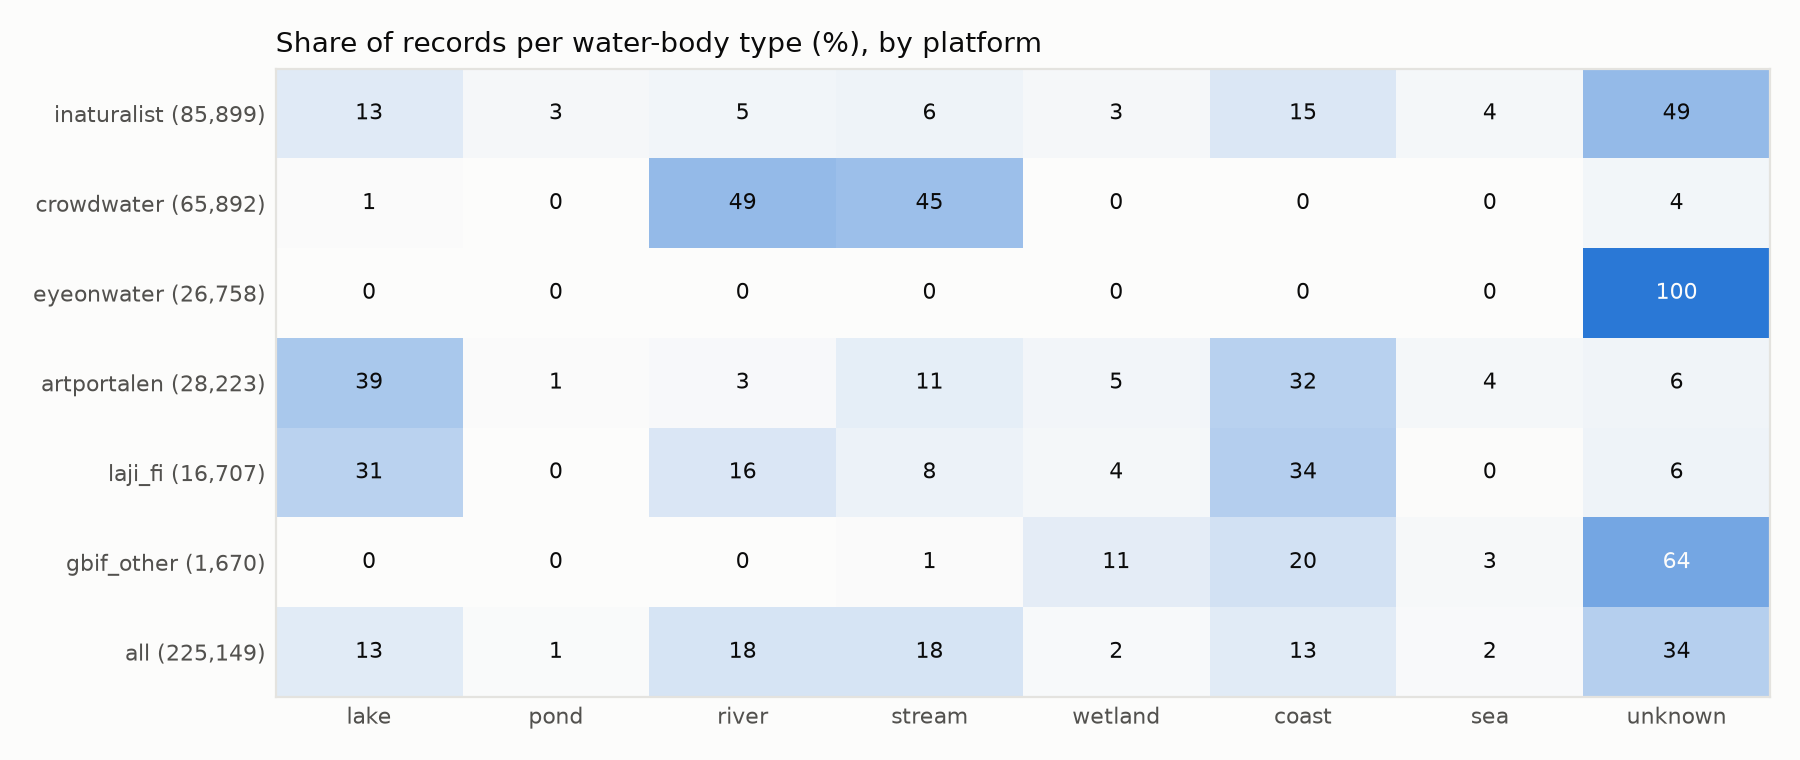
\includegraphics[width=\columnwidth]{stats_water_body_by_platform.png}
\caption{Share of records per water-body type and platform (\%).}
\label{fig:waterbody}
\end{figure}

\section{Spec 3 --- Corpus statistics}

Table~\ref{tab:corpus} compares the notes with the Brown~\cite{francis1979brown} and
Reuters-21578~\cite{lewis1997reuters} corpora. The notes are rather short, and many words are only seen once. Their higher
WordNet~\cite{miller1995wordnet} coverage comes from missing function words. FinnWordNet~\cite{linden2010finnwordnet}
covers 72\% of Finnish tokens.

\begin{table}[htbp]
\centering\small
\caption{Field notes vs edited text.}
\label{tab:corpus}
\resizebox{\columnwidth}{!}{%
\begin{tabular}{lrrr}
\toprule
 & Field notes & Brown & Reuters \\
\midrule
Mean length (tokens) & 3.2 -- 12.4 & 17.5 & 24.3 \\
Median length & 2 -- 7 & 15 & 23 \\
Words seen once & 49 -- 61\% & 43\% & 36\% \\
Types in 25k tokens & 4{,}622 -- 5{,}910 & 6{,}327 & 4{,}448 \\
Number tokens & 5 -- 15\% & 1\% & 10\% \\
WordNet coverage (English) & 76 -- 82\% & 70\% & 74\% \\
\bottomrule
\end{tabular}}
\end{table}

\section{Spec 4 --- Zipf and Heaps}

\textbf{Zipf}~\cite{zipf1949human}: OLS of log frequency on log rank, with the 90\% confidence interval of the slope,
$R^2$ and adjusted $R^2$ (Table~\ref{tab:zipf-platform}, Figure~\ref{fig:zipf}). The law holds ($R^2$ 0.95--0.98, like
Brown and Reuters).

\begin{table}[htbp]
\centering
\small
\caption{Zipf fits by platform (spec 4): OLS of $\log_{10}$ frequency on $\log_{10}$ rank with 90\% confidence interval of the slope.}
\label{tab:zipf-platform}
\resizebox{\linewidth}{!}{%
\begin{tabular}{lrrrrrrr}
\toprule
platform & types & slope & 90\% lo & 90\% hi & $R^2$ & adj. $R^2$ & slope top-1000 \\
\midrule
inaturalist & 16{,}209 & -1.289 & -1.292 & -1.287 & 0.973 & 0.973 & -0.952 \\
artportalen & 19{,}372 & -1.157 & -1.160 & -1.154 & 0.954 & 0.954 & -1.015 \\
crowdwater & 13{,}376 & -1.087 & -1.090 & -1.084 & 0.963 & 0.963 & -0.952 \\
laji\_fi & 9{,}511 & -0.972 & -0.976 & -0.968 & 0.950 & 0.950 & -0.949 \\
Brown & 47{,}039 & -1.323 & -1.325 & -1.321 & 0.974 & 0.974 & -0.977 \\
Reuters & 29{,}188 & -1.557 & -1.560 & -1.555 & 0.978 & 0.978 & -0.961 \\
\bottomrule
\end{tabular}
}
\end{table}


\begin{figure}[htbp]
\centering
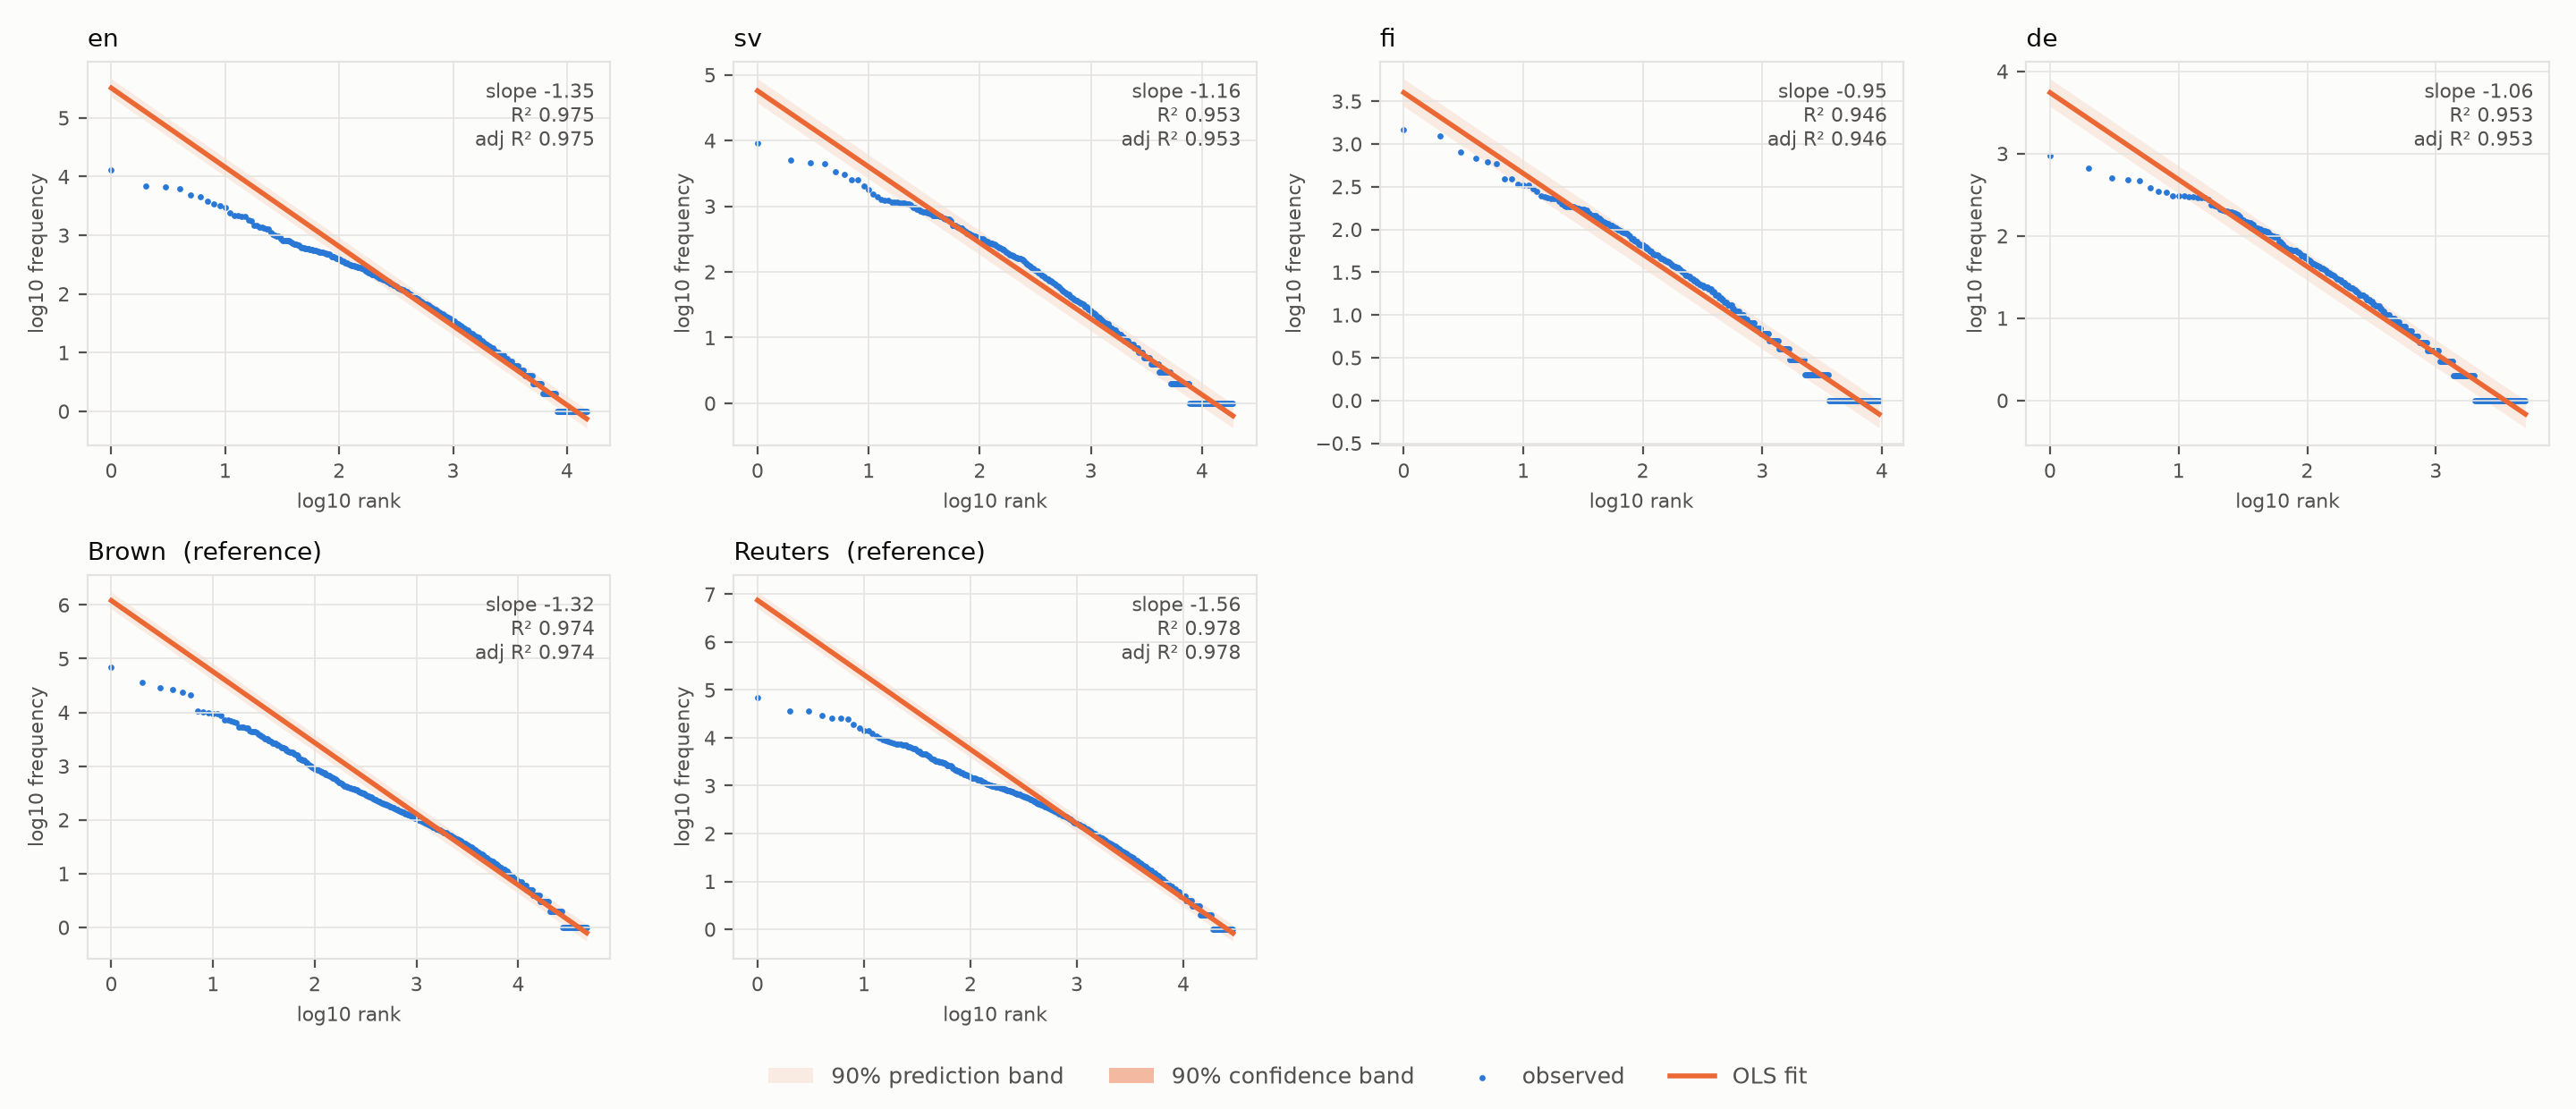
\includegraphics[width=\textwidth]{spec4_zipf_by_language.png}
\caption{Zipf plots by language with OLS fit, 90\% confidence band (dark) and 90\% prediction band (light).}
\label{fig:zipf}
\end{figure}

\textbf{Heaps}~\cite{heaps1978information}: vocabulary size $V$ at every 5\% of the tokens and is fitted as $V = K N^\beta$
(Table~\ref{tab:heaps-platform}, Figure~\ref{fig:heaps}). Here, the field notes grow faster ($\beta$ 0.55--0.68) than Brown
(0.51) and Reuters (0.45). 

\begin{table}[htbp]
\centering
\small
\caption{Heaps fits by platform (spec 4): $V = K N^\beta$ on vocabulary sizes at every 5\% of the tokens.}
\label{tab:heaps-platform}
\begin{tabular}{lrrrrrrr}
\toprule
platform & tokens & types & $K$ & $\textbackslash{}beta$ & 90\% lo & 90\% hi & $R^2$ \\
\midrule
inaturalist & 246{,}659 & 16{,}209 & 17.92 & 0.549 & 0.543 & 0.555 & 0.999 \\
artportalen & 224{,}669 & 19{,}372 & 8.71 & 0.626 & 0.623 & 0.629 & 1.000 \\
crowdwater & 103{,}315 & 13{,}376 & 10.37 & 0.622 & 0.616 & 0.628 & 1.000 \\
laji\_fi & 52{,}767 & 9{,}511 & 7.78 & 0.654 & 0.651 & 0.658 & 1.000 \\
Brown & 1{,}006{,}060 & 47{,}039 & 44.82 & 0.505 & 0.494 & 0.516 & 0.997 \\
Reuters & 1{,}330{,}267 & 29{,}188 & 55.22 & 0.446 & 0.439 & 0.454 & 0.998 \\
\bottomrule
\end{tabular}
\end{table}

\begin{table}[htbp]
\centering
\small
\caption{New word types added in selected 5\% steps of tokens, and the ratio of the last to the first step: growth slows down, much less for field notes than for edited text.}
\label{tab:heaps-inc}
\begin{tabular}{lrrrrrrr}
\toprule
 & 5\% & 10\% & 25\% & 50\% & 75\% & 100\% & last/first \\
\midrule
inaturalist & 3{,}065 & 1{,}520 & 870 & 596 & 442 & 415 & 0.14 \\
artportalen & 2{,}951 & 1{,}622 & 1{,}091 & 812 & 694 & 607 & 0.21 \\
crowdwater & 2{,}075 & 1{,}212 & 818 & 610 & 449 & 358 & 0.17 \\
laji\_fi & 1{,}326 & 786 & 496 & 378 & 332 & 332 & 0.25 \\
Brown & 9{,}939 & 5{,}227 & 2{,}668 & 1{,}709 & 1{,}292 & 1{,}023 & 0.10 \\
Reuters & 7{,}508 & 3{,}143 & 1{,}621 & 952 & 750 & 548 & 0.07 \\
\bottomrule
\end{tabular}
\end{table}


\begin{figure}[htbp]
\centering
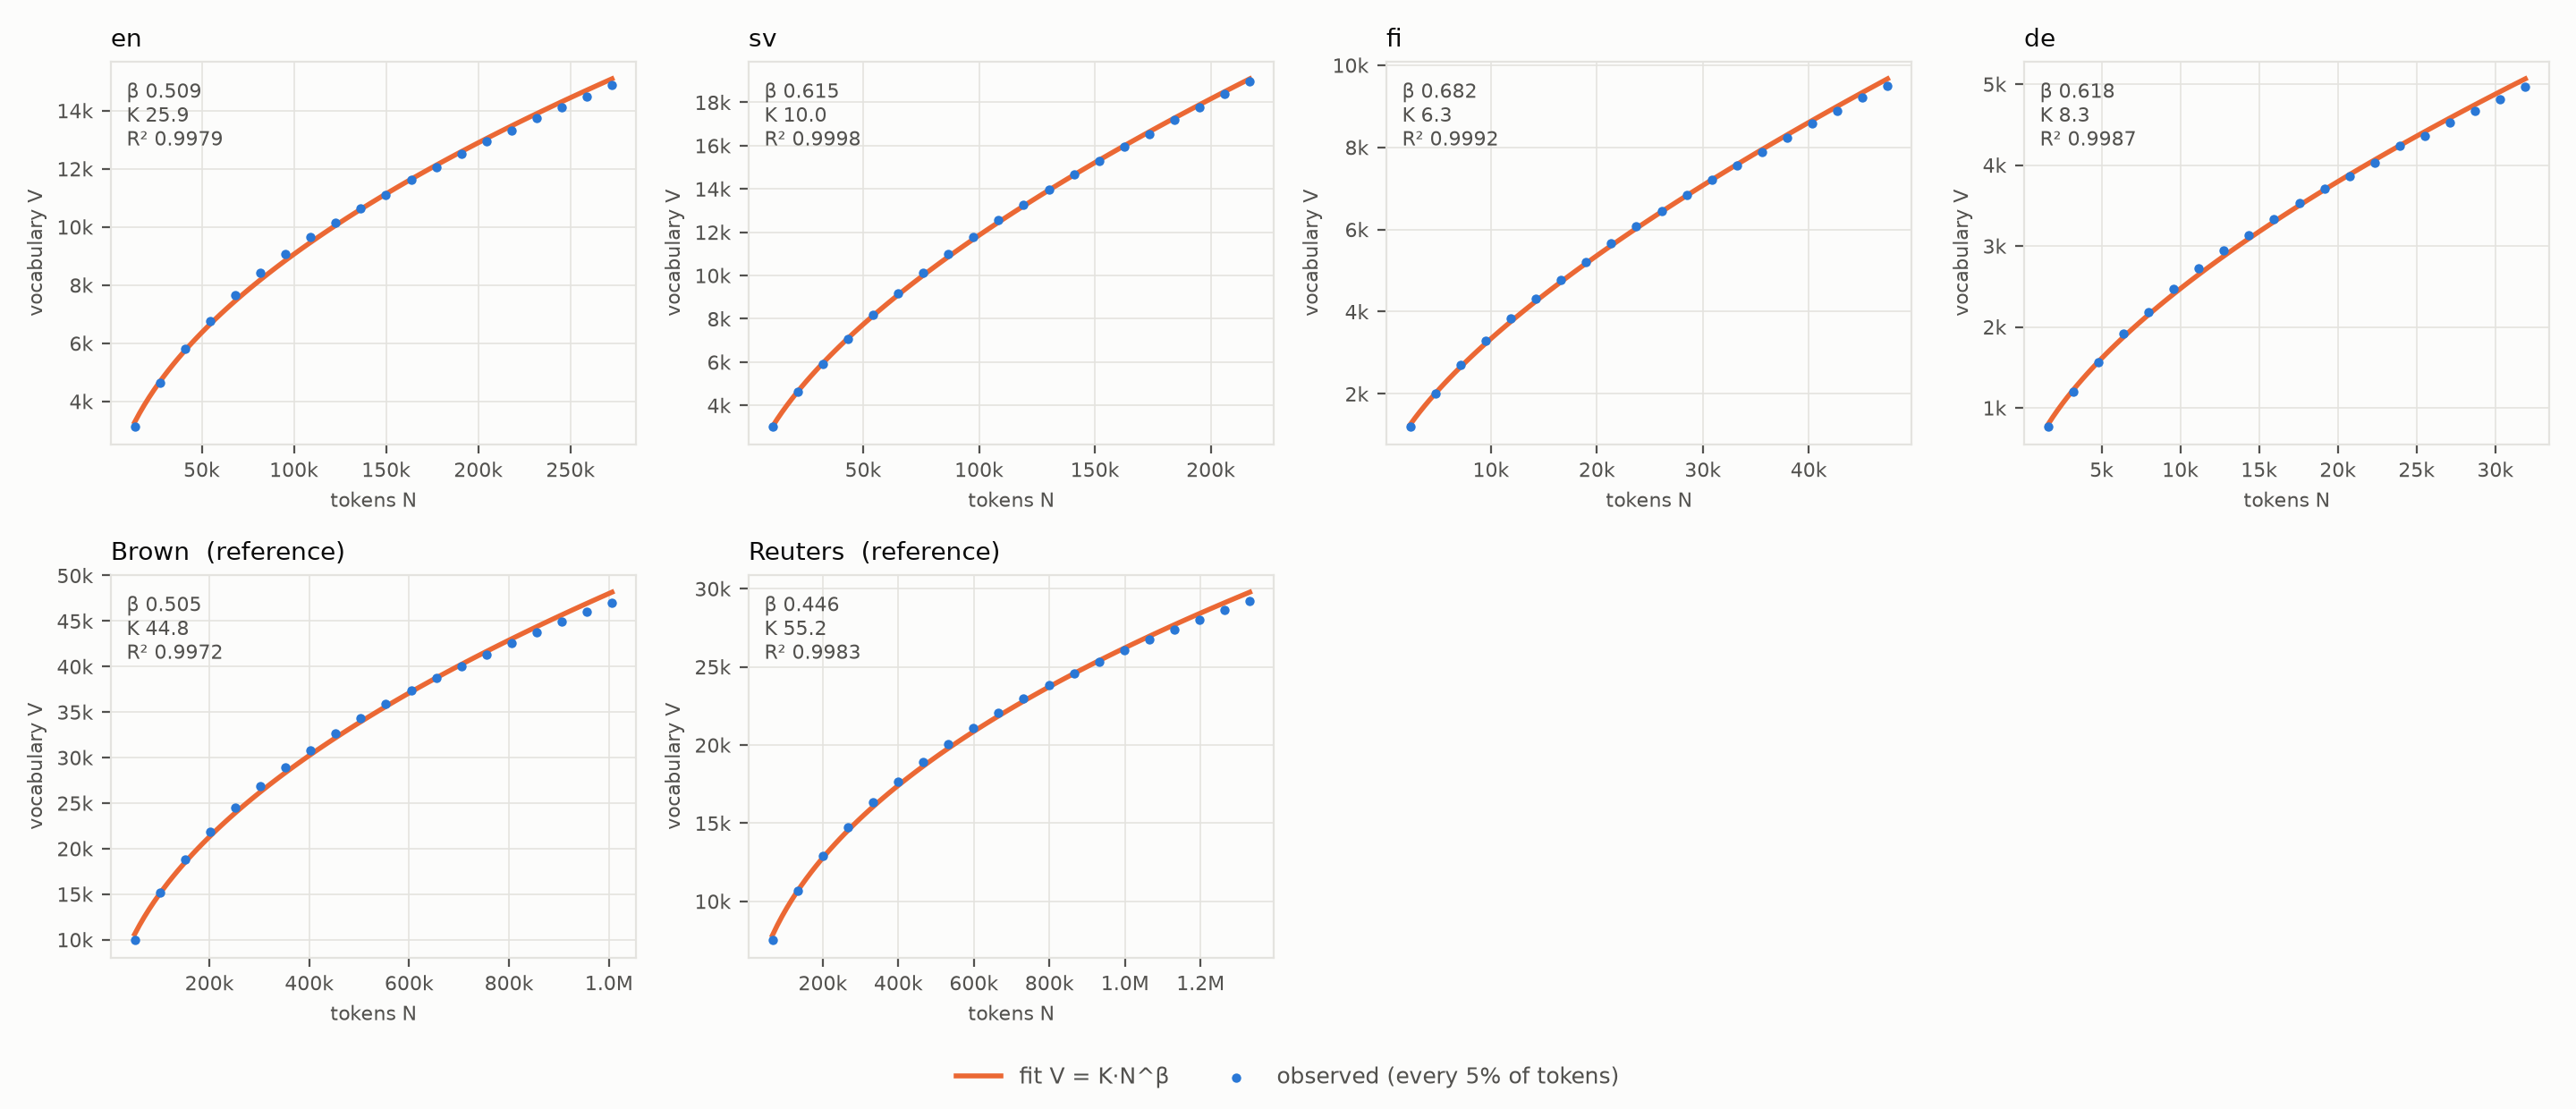
\includegraphics[width=0.78\textwidth]{spec4_heaps_by_language.png}
\caption{Heaps curves by language: vocabulary size against tokens, with fitted $V = K N^\beta$.}
\label{fig:heaps}
\end{figure}

\section{Spec 5 --- Information extraction}

We extract six entity types (water body, location, organism, quantity, date/time, weather) and twelve water conditions
with three systems: spaCy pipelines for 18 languages~\cite{honnibal2020spacy}, a multilingual XLM-RoBERTa NER
model~\cite{conneau2020xlmr}, and our rules (water-term lists in nine languages and regular expressions). The NER
models know places, dates and numbers but not organisms, water bodies or weather, which only the rules cover. The
same NER output was used to mask personal names: 8.8\% of notes named a person, mostly survey credits.

\section{Spec 6 --- Gold set}

We labelled 300 records from one stratified sample, plus 20 calibration records labelled by
all three of us. Each gold record was labelled by one student and one LLM
(Qwen2.5-VL-7B~\cite{bai2025qwen25vl}) and a third person decided the disagreements. Table~\ref{tab:gold} summarises the
labels.

\begin{table}[htbp]
\centering\small
\caption{Gold set (300 records).}
\label{tab:gold}
\resizebox{\columnwidth}{!}{%
\begin{tabular}{ll}
\toprule
Label & Distribution \\
\midrule
Relevance & about water 150, not 134, uncertain 16 \\
Conditions & none stated 128; low or dry 16, high water 7, clear 6, turbid 4 \\
Entities (144 spans) & water body 54, quantity 28, weather 18, location 16, organism 15, date 13 \\
Image--text & consistent 94, cannot judge 11, inconsistent 5, partly 3 \\
\bottomrule
\end{tabular}}
\end{table}

\section{Spec 7 --- Agreement and extractor evaluation}

The agreement is measured with Cohen's $\kappa$~\cite{cohen1960kappa} and span F1 (Table~\ref{tab:agreement}). 
The agreement between us students was high, but the agreement with the LLM is low - 68\% of notes got marked as ``not about water'', 
while we students only labelled 40\% this way.

\begin{table}[htbp]
\centering\small
\caption{Agreement: relevance and condition $\kappa$, span F1 (exact / partial).}
\label{tab:agreement}
\resizebox{\columnwidth}{!}{%
\begin{tabular}{lrrr}
\toprule
Pair & Relevance $\kappa$ & Conditions $\kappa$ & Span F1 \\
\midrule
Students, calibration (20) & 0.80 & 1.00 & 1.00 / 1.00 \\
Student vs LLM, gold (300) & 0.25 & 0.29 & 0.20 / 0.29 \\
\bottomrule
\end{tabular}}
\end{table}

The extractors are scored on the gold entity spans (Table~\ref{tab:extractors}). Exact scores are low because span
boundaries differ from the guideline. With partial matching the rules are best.
For water conditions the rules reach F1 0.31 (precision 0.50, recall 0.22). Only 51\% of the
gold notes are actually about water. Translating non-English notes to English helps condition extraction but
hurts entity extraction, because translation garbles names and abbreviations (Table~\ref{tab:mt}).

\begin{table}[htbp]
\centering\small
\caption{Extractors on the gold set (150 spans, micro F1).}
\label{tab:extractors}
\begin{tabular}{lrrr}
\toprule
System & F1 exact & F1 partial & Predicted \\
\midrule
spaCy & 0.20 & 0.34 & 96 \\
XLM-R NER & 0.20 & 0.28 & 65 \\
Rules & 0.12 & \textbf{0.44} & 210 \\
Union & \textbf{0.22} & 0.40 & 332 \\
\bottomrule
\end{tabular}
\end{table}

\begin{table}[htbp]
\centering\small
\caption{Extraction F1 on English originals vs non-English notes, original and machine-translated.}
\label{tab:mt}
\resizebox{\columnwidth}{!}{%
\begin{tabular}{lrrr}
\toprule
Text & spaCy entities & Rules entities & Rules conditions \\
\midrule
English originals & 0.42 & 0.53 & 0.39 \\
Non-English, original & 0.28 & 0.37 & 0.22 \\
Non-English, translated & 0.18 & 0.32 & 0.37 \\
\bottomrule
\end{tabular}}
\end{table}

\section{Spec 8 --- Weak-label baselines}

Using just the note, we can predict the Artportalen habitat field, as well as the CrowdWater water-level class.
The dataset was split 80/10/10, stratified by platform; each CrowdWater gauge was kept in one split, which results in a 64/8/28 split for CrowdWater.
Due to EyeOnWater having no notes, we cannot predict its Forel-Ule colour field from text.
The models used were a TF-IDF with a linear SVM, and a multilingual DistilBERT~\cite{sanh2019distilbert}, with and without stopwords (Table~\ref{tab:weak}). 


\begin{table}[htbp]
\centering\small
\caption{Weak-label baselines, test macro F1 (117 habitat, 578 water-level notes).}
\label{tab:weak}
\begin{tabular}{lrr}
\toprule
Model & Habitat & Water level \\
\midrule
Majority class & 0.05 & 0.04 \\
TF-IDF + SVM & \textbf{0.73} & \textbf{0.22} \\
DistilBERT & 0.65 & 0.15 \\
\bottomrule
\end{tabular}
\end{table}

From the results, we can see that habitat is much easier to predict from the note than water level.
This is thanks to the fact that habitat is often mentioned in the note; while water level is not, since it is read from a gauge in the photo.
A surprising result is that the simple SVM had superior performance to DistilBERT, which is a much more complex model.
Removing stopwords didn't affect much the performance of the models, with the macro f1 score changing by less than 0.01 in all cases.

\section{Spec 9 --- Image--text consistency}

We compare each note against its photo with the cosine similarity of CLIP~\cite{radford2021clip} (English text) and
multilingual SigLIP~\cite{zhai2023siglip} embeddings, on 148 gold records with a photo, as well as 600 other pairs. 
Due to only 8 gold records being inconsistent, we decided to score as well each note against a different, random record's photo, 
with the expectation being that a useful model should prefer the real pair (Table~\ref{tab:clip}, Figure~\ref{fig:clip}).

\begin{table}[htbp]
\centering\small
\caption{Image--text similarity: AUC of own vs another photo, and against the gold labels.}
\label{tab:clip}
\resizebox{\columnwidth}{!}{%
\begin{tabular}{lrrrr}
\toprule
Model & Own vs other & iNaturalist & CrowdWater & Gold (consistent vs not) \\
\midrule
CLIP (English) & 0.72 & 0.80 & 0.64 & 0.73 \\
SigLIP (original) & 0.70 & 0.75 & 0.66 & 0.70 \\
SigLIP (translation) & 0.69 & 0.75 & 0.63 & 0.71 \\
\bottomrule
\end{tabular}}
\end{table}

\begin{figure}[htbp]
\centering
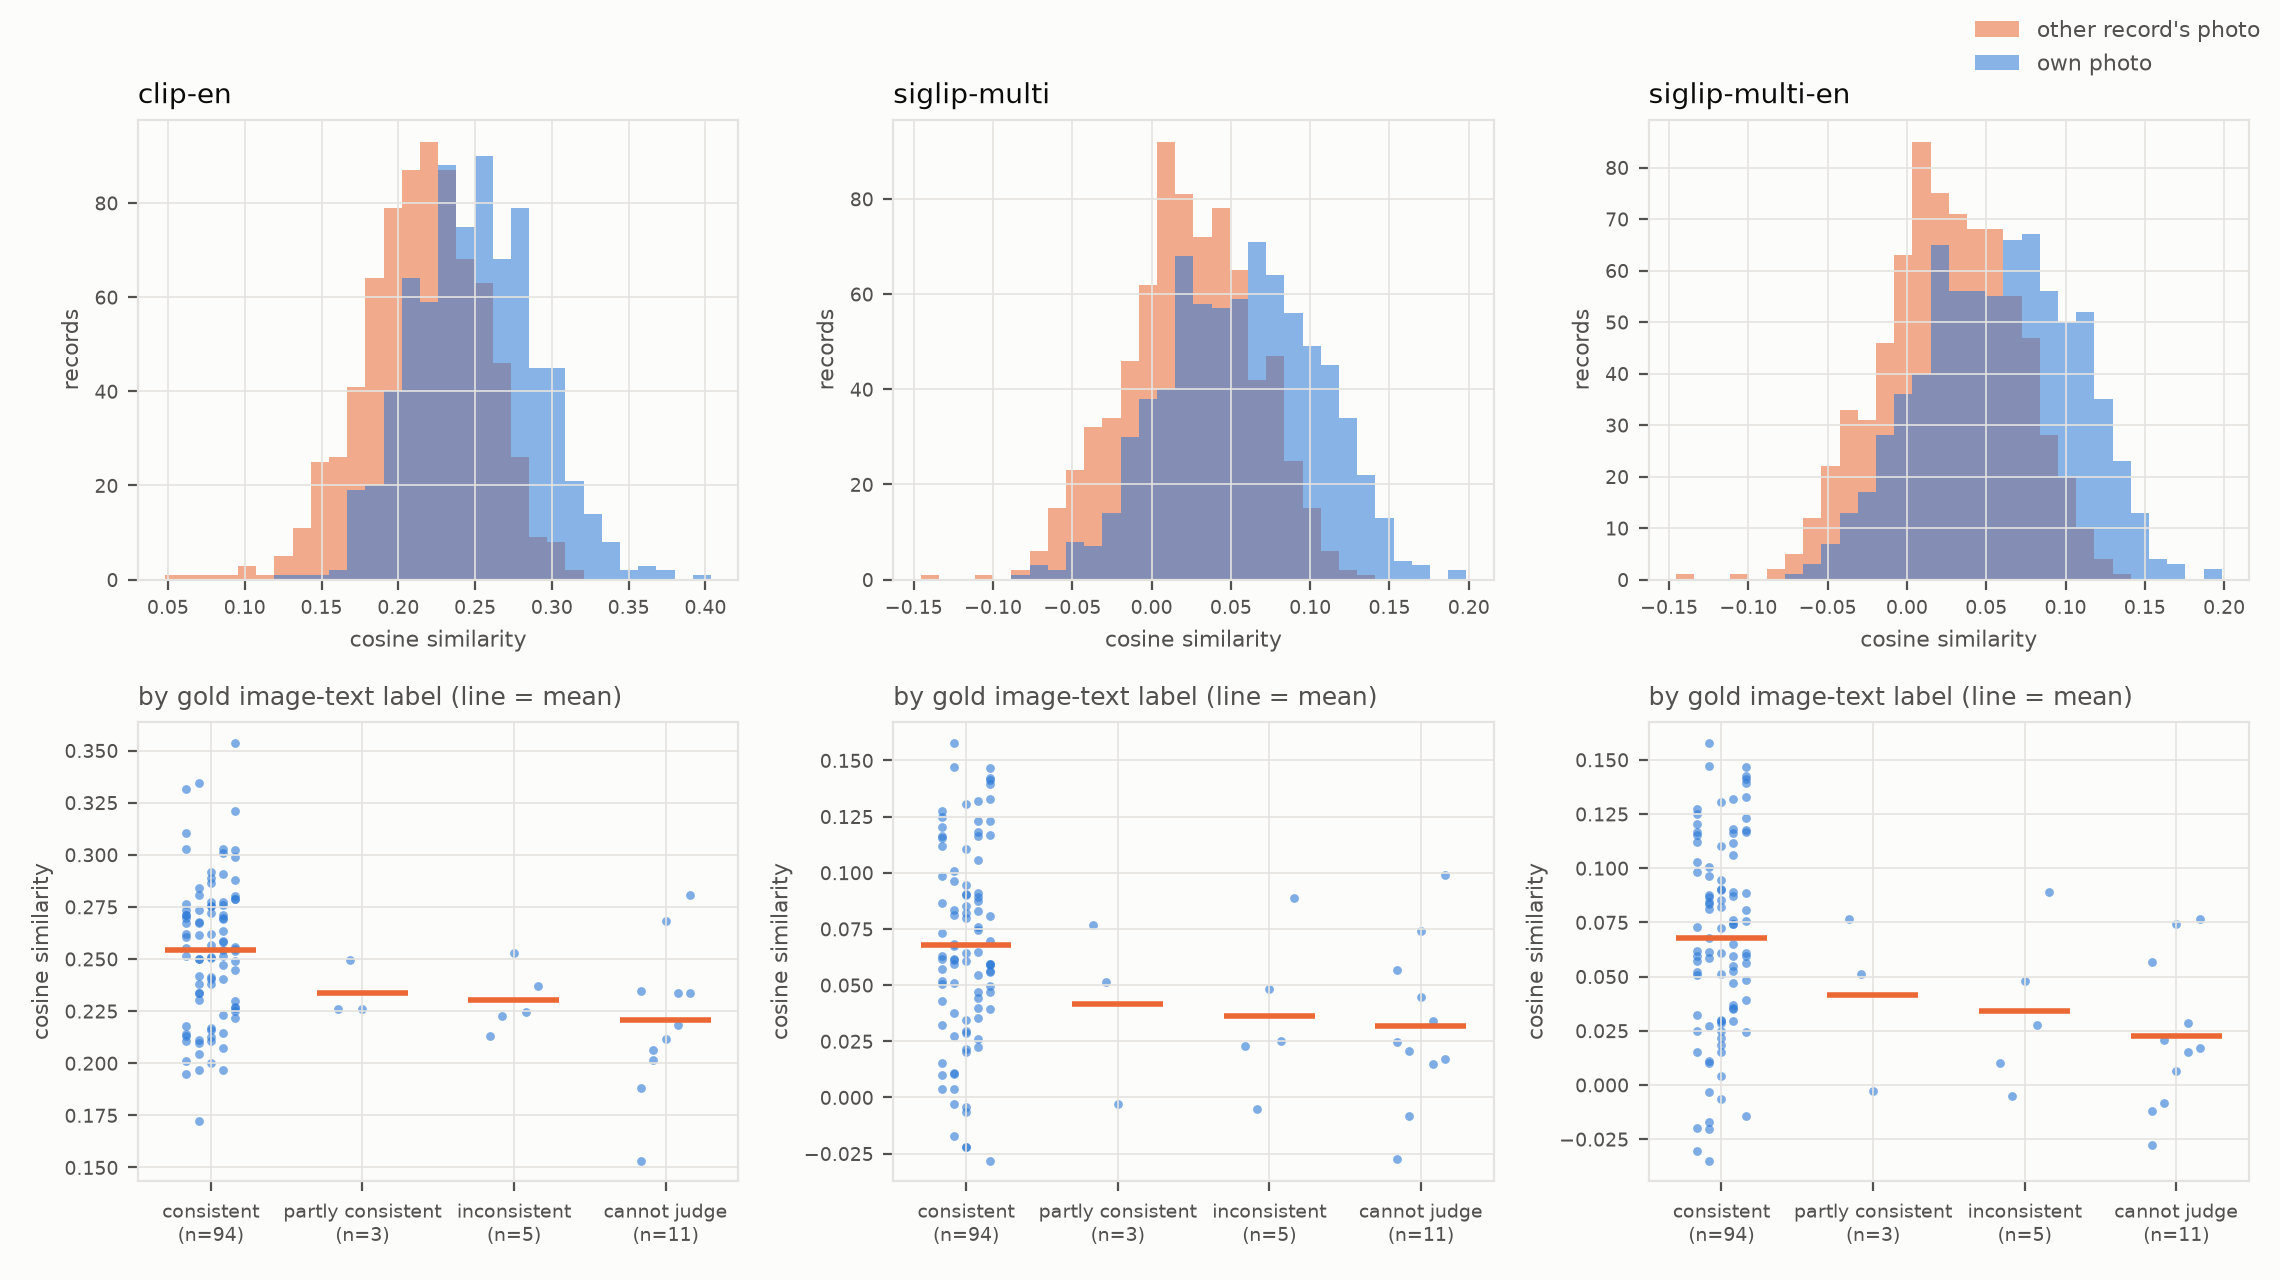
\includegraphics[width=0.85\textwidth]{spec9_similarity.png}
\caption{Similarity of a note with its own photo vs another record's photo (top) and by gold label (bottom).}
\label{fig:clip}
\end{figure}

From the results we can conclude that the real pair is preferred about 75\% of the time, which is to say about 3 times in 4.
This score is well above random chance, but it is not reliable. It works well on iNaturalist, where the note names the species in the photo,
but quite poorly on CrowdWater where all photos show a riverbank with a gauge. This is due to the fact that the models measure whether photo and note 
are about the same topic, but not whether the photo shows the condition the note describes.
\section{Spec 11 --- Bias audit}

\begin{table}[htbp]
\centering\small
\caption{Bias audit summary (Gini: 0 = equal, 1 = one unit has everything).}
\label{tab:bias}
\begin{tabular}{lp{0.68\columnwidth}}
\toprule
Dimension & Finding \\
\midrule
Geography & 148 countries; Sweden, US and Switzerland hold 37\% of records (Gini 0.91); Africa, South Asia and South
America nearly absent; Latvia only 264 records. \\
Language & Swedish, English and Finnish are 72\% of the notes (Gini 0.82). \\
Season & Summer 37\%, spring 29\%, autumn 20\%, winter 15\%. \\
Users & The top 1\% of users wrote 20--61\% of a platform's records (Gini 0.65--0.88); CrowdWater has no user id. \\
\bottomrule
\end{tabular}
\end{table}

The corpus is significantly biased (Table~\ref{tab:bias}, Figures~\ref{fig:map} and~\ref{fig:months}). 
This is partly a result of our own collection choices, since iNaturalist was collected for 14 countries and three sources are national portals.
Only CrowdWater and EyeOnWater are global. Records peak mostly in summer, meaning that winter states such as ice are rare (only two gold records).
Additionally, on Laji.fi, about nine people (the top 1\% of users) wrote 61\% of the records, so in the Finnish text, the abbreviations they
use dominate. This means that the results on CSWO-Bench should be reported per platform and language, and shouldn't be transferred to other regions, 
seasons or languages without previous analysis.



\begin{figure}[htbp]
\centering
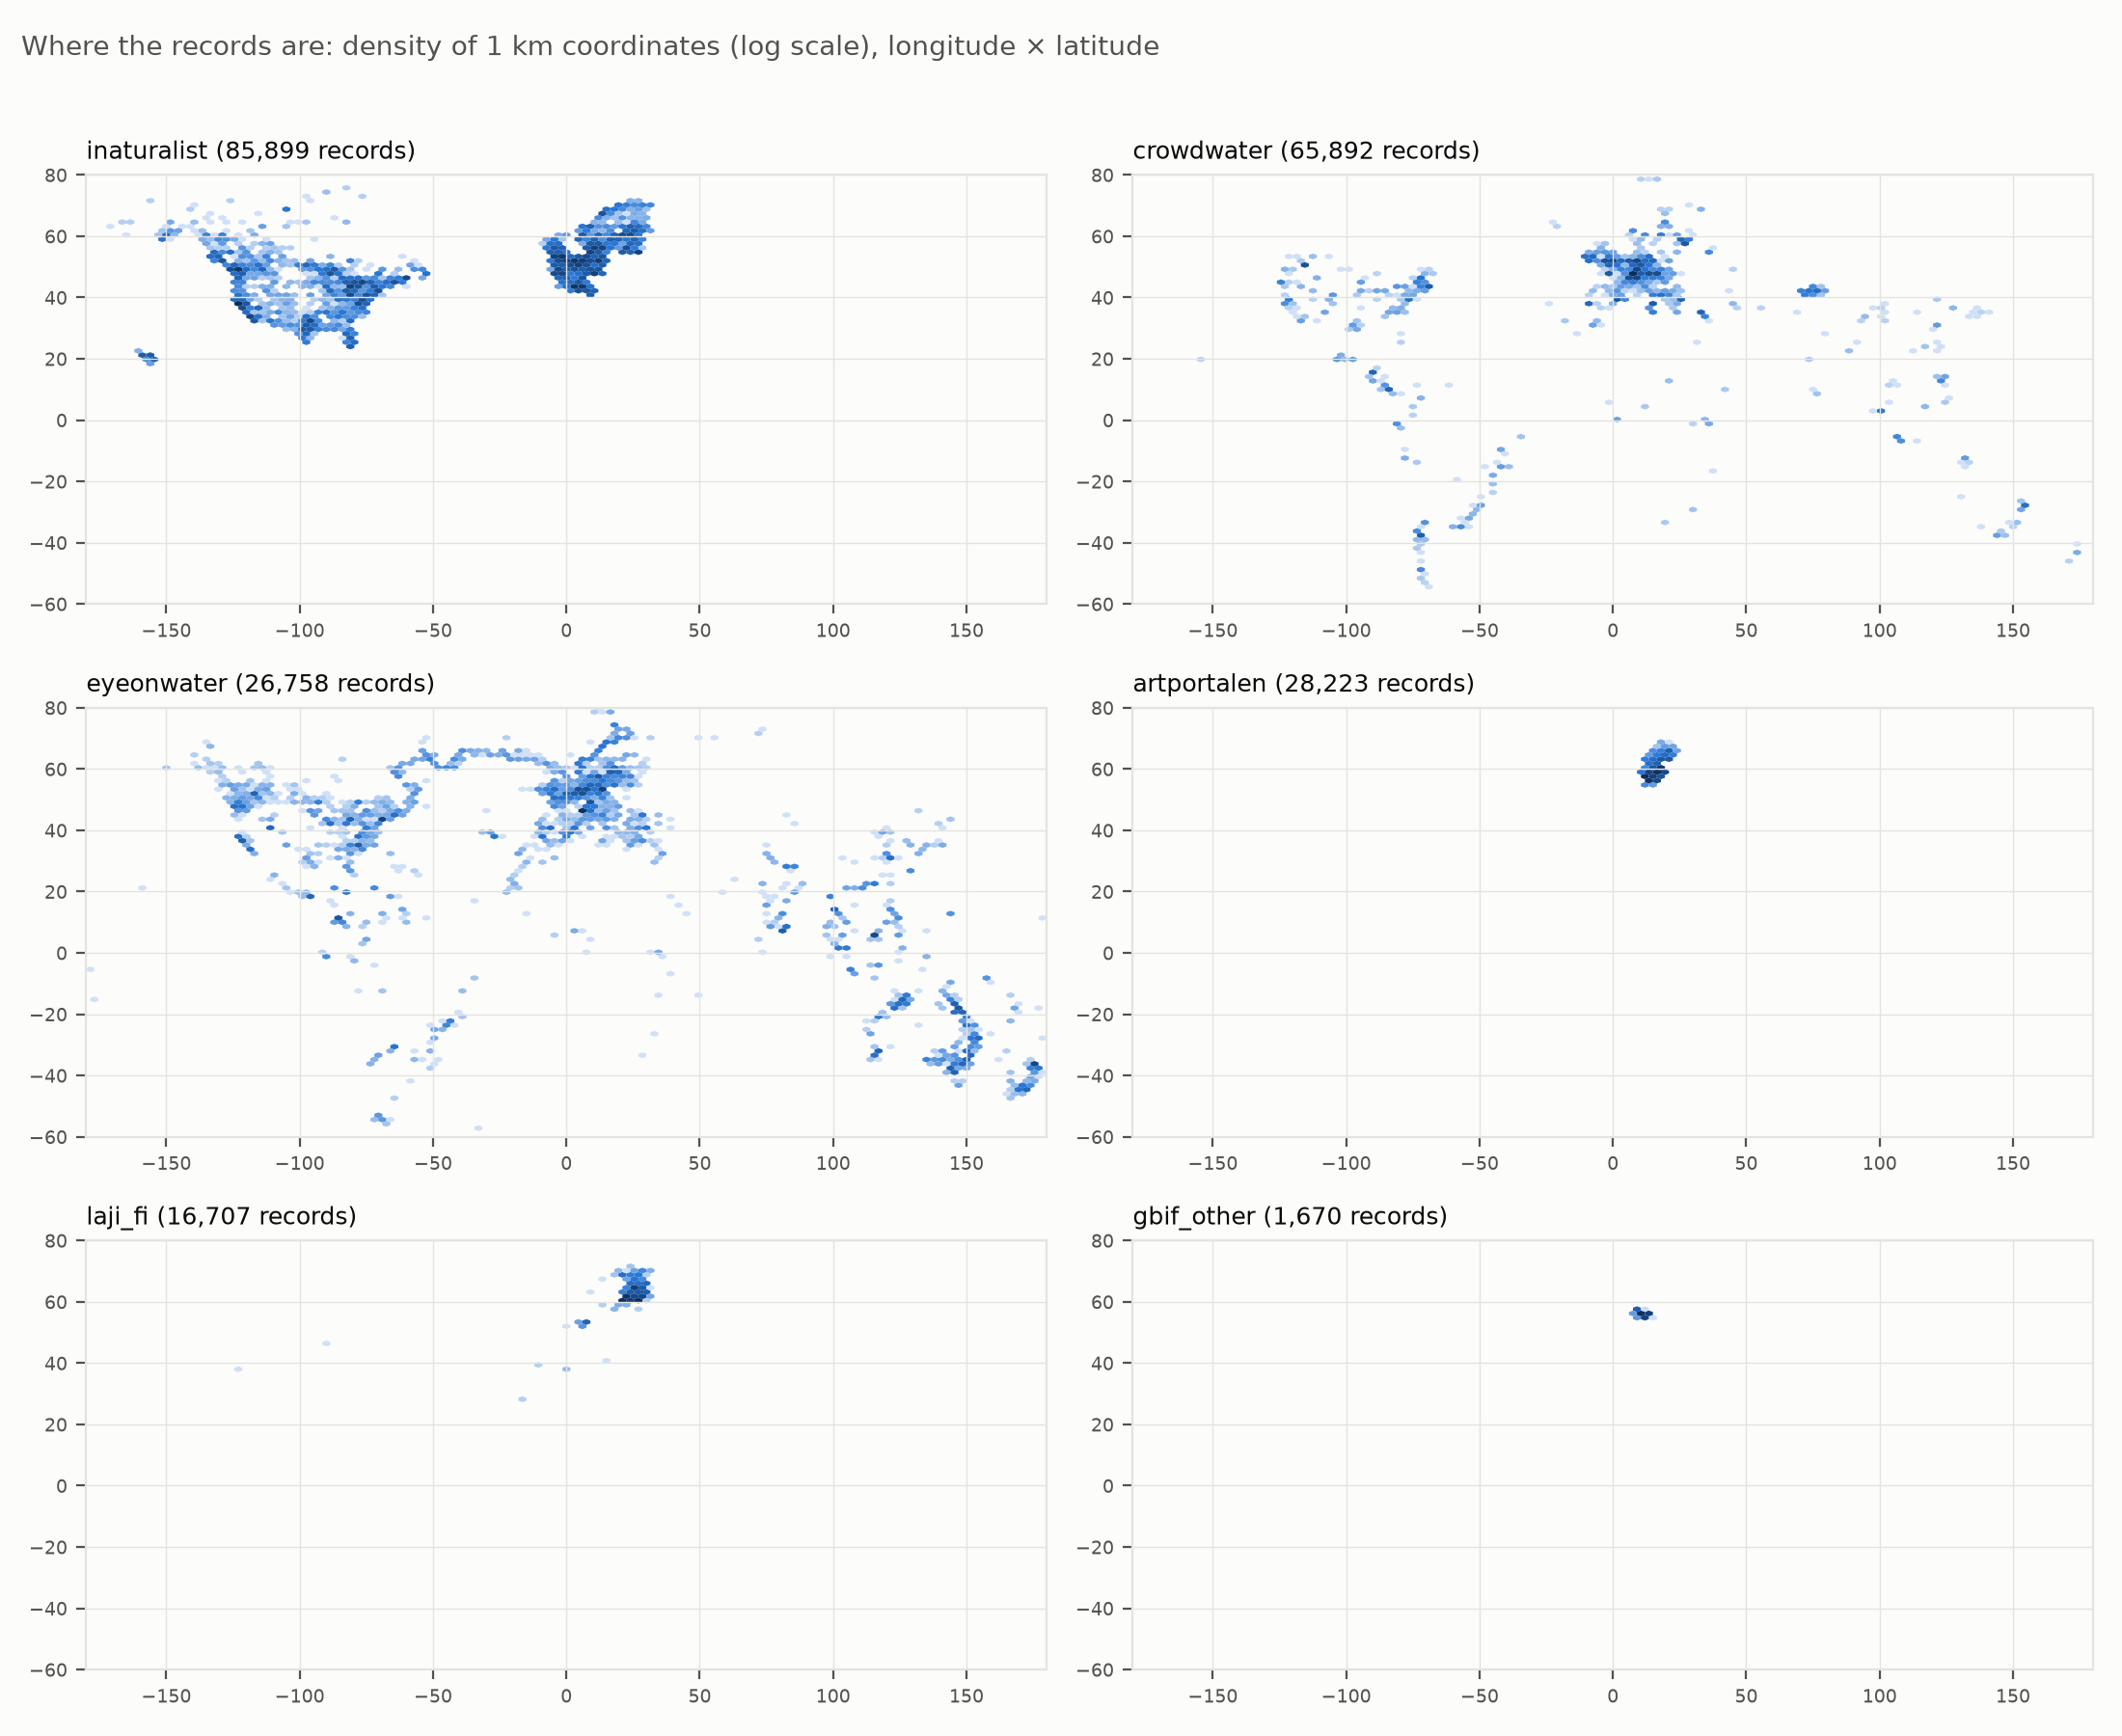
\includegraphics[width=0.72\textwidth]{spec11_map.png}
\caption{Where the records are: density of coordinates per platform (longitude $\times$ latitude).}
\label{fig:map}
\end{figure}

\begin{figure}[htbp]
\centering
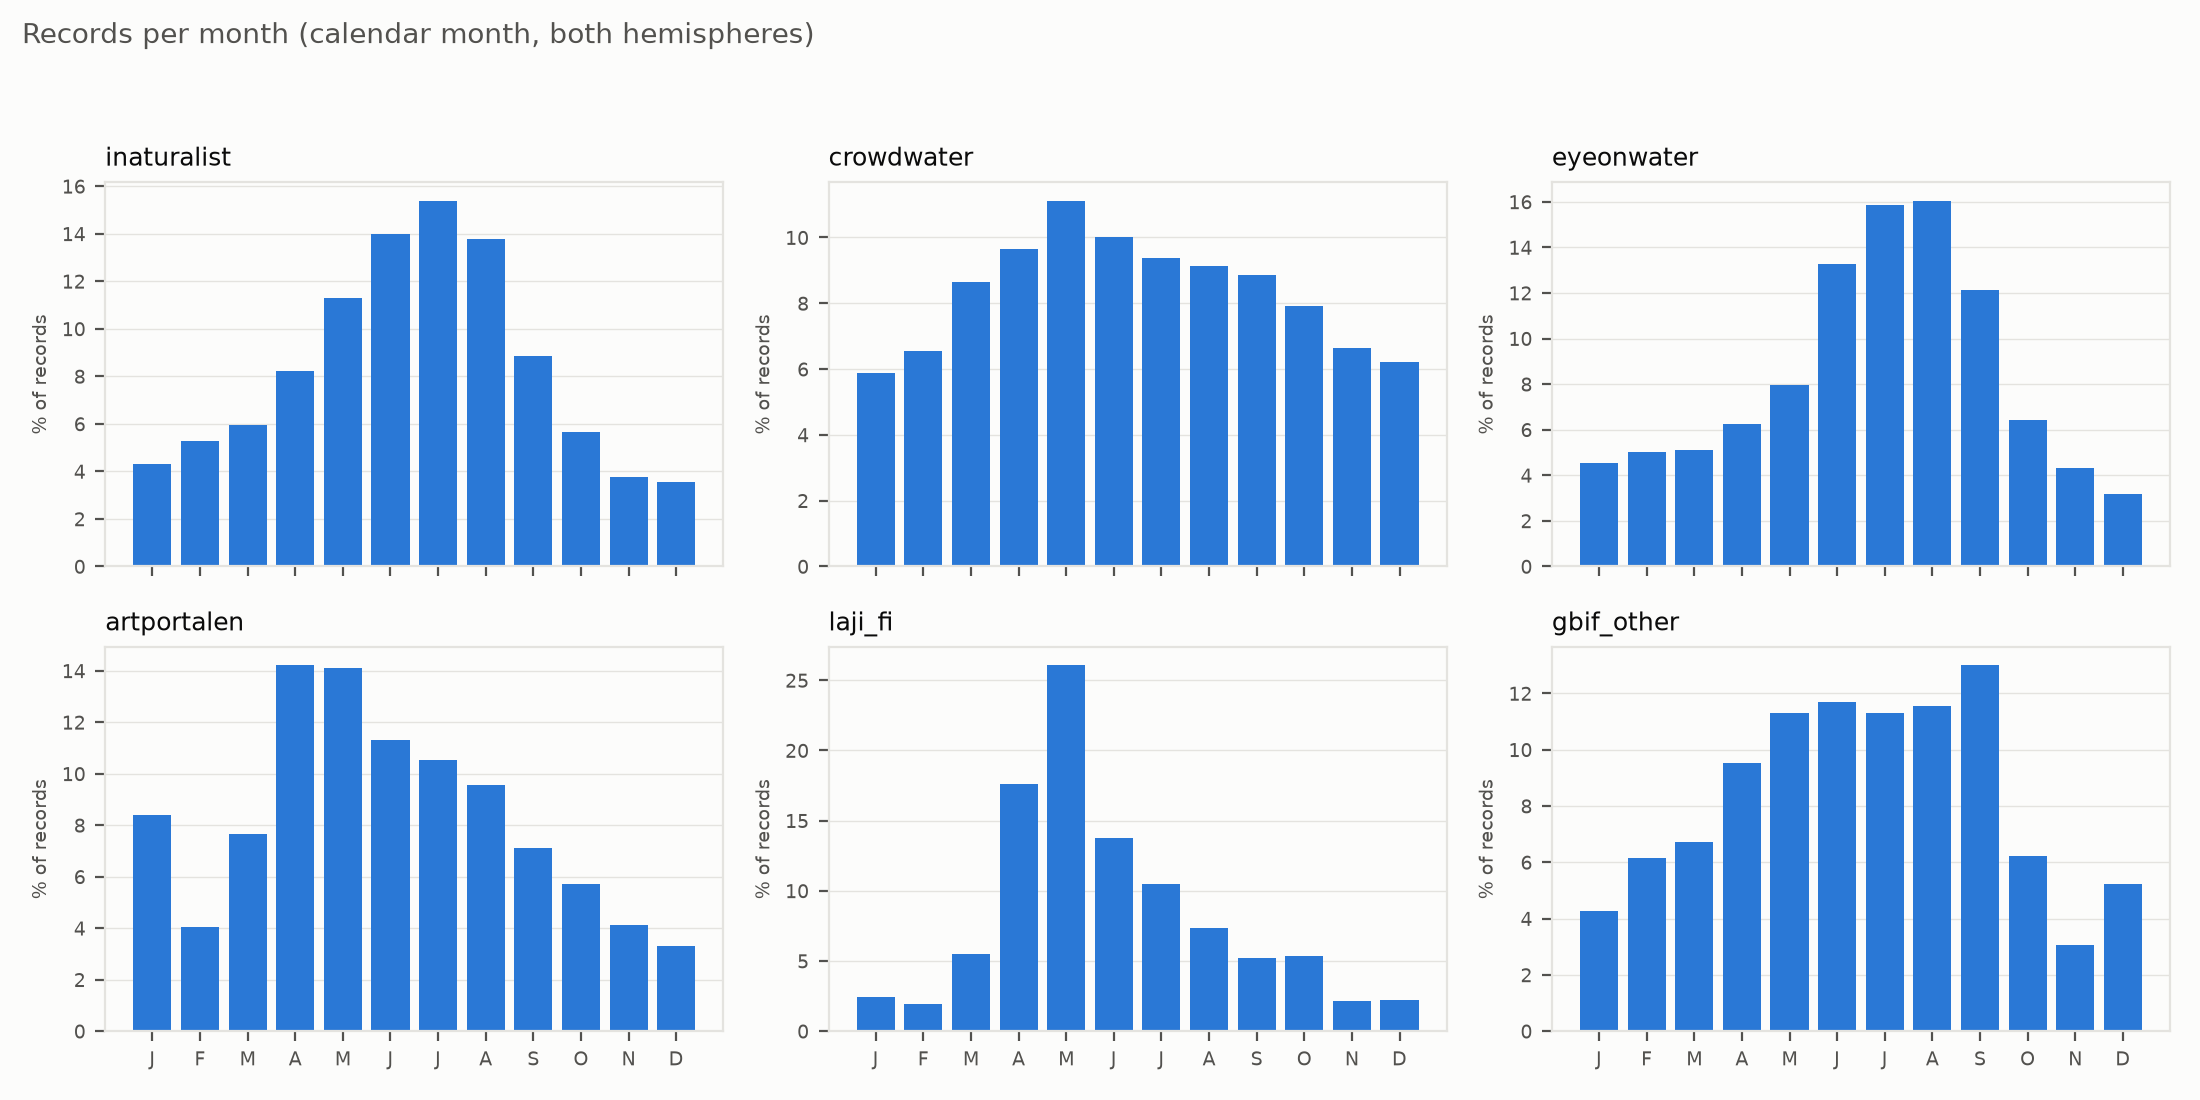
\includegraphics[width=\columnwidth]{spec11_months.png}
\caption{Share of records per calendar month, by platform.}
\label{fig:months}
\end{figure}

\section{Spec 14 --- Literature and limitations}

\textbf{Literature.} CrowdWater's virtual staff gauges~\cite{seibert2019crowdwater} and GBIF's national
portals~\cite{gbif} provide the structured data we build on; Kosmala et al.~\cite{kosmala2016quality} show that
citizen-science data can be reliable when quality is checked, which motivates our gold set and bias audit.
Our statistics follow Zipf~\cite{zipf1949human} and Heaps~\cite{heaps1978information}; agreement uses Cohen's
$\kappa$~\cite{cohen1960kappa}; the data card follows Datasheets for Datasets~\cite{gebru2021datasheets}. Beyond specs
2--9, the repository also contains a zero-shot LLM/VLM evaluation (Qwen2.5~\cite{qwen2024qwen25,bai2025qwen25vl};
68--69\% of checked outputs hallucinate, in the sense of~\cite{ji2023hallucination}) and a GLiNER
comparison~\cite{zaratiana2024gliner} that raises partial entity F1 from 0.44 to 0.52.


\textbf{Limitations.}
\begin{itemize}
  \item \emph{Gold design:} one student and one LLM per record (course guideline), not two students; student--student
        agreement comes only from the 20 calibration records.
  \item \emph{Split:} CrowdWater is 64/8/28 instead of 80/10/10, to keep each gauge in one split.
  \item \emph{Small numbers:} few positive gold labels (5 inconsistent image--text pairs, 4 turbid notes).
  \item \emph{Pipeline errors:} language identification fails on species names; translations are plausible but not
        always correct; the water filter is keyword-based (only 51\% of gold notes are about water).
  \item \emph{Coverage and privacy:} Latvian data is almost absent (non-commercial licences excluded); name masking
        misses a few names; photos are linked, not copied.
\end{itemize}

\section{Code availability}
\label{sec:code}

All source code, the fixed splits, the gold labels, the results and the data card are in the repository
\url{https://github.com/notEloiMm/cswo-bench} (MIT licence for the code). The pipeline is a Python package
(\texttt{src/cswo/}) with one command per step listed in the README. The steps that need a GPU
are Jupyter notebooks in \texttt{notebooks/} that run on a free Google Colab T4:
\begin{itemize}
  \item \texttt{colab\_translate.ipynb} --- translation to English (spec 2);
  \item \texttt{colab\_llm\_annotate.ipynb} --- LLM second annotator for the gold set (spec 6);
  \item \texttt{colab\_bert.ipynb} --- DistilBERT baselines (spec 8);
  \item \texttt{colab\_clip.ipynb} --- CLIP/SigLIP image--text similarity (spec 9);
  \item \texttt{colab\_zeroshot.ipynb} --- zero-shot LLM/VLM evaluation (spec 10).
\end{itemize}
The evaluation scripts read only committed files (gold labels, extractor outputs, model predictions), so every table
of this report can be reproduced without the full corpus.

\section{Use of AI tools}
\label{sec:ai}

\paragraph{AI assistance in producing the project.} 
We used LLMs in different context throughout the project. 
We used Claude for generating tedious coding tasks and autocompletion - always supervised. It was also used as help for plotting plots.  Further we used it for generating scripts and the 
generation of latex tables - with Gemini. 


\bibliographystyle{plain}
\bibliography{references}

\end{document}
